\documentclass[../rapport.tex]{subfiles}
\graphicspath{{\subfix{ressources/photos_diagrammes/}}}
\newpage

\begin{document}
	
	\begin{figure}[h]
		\centering 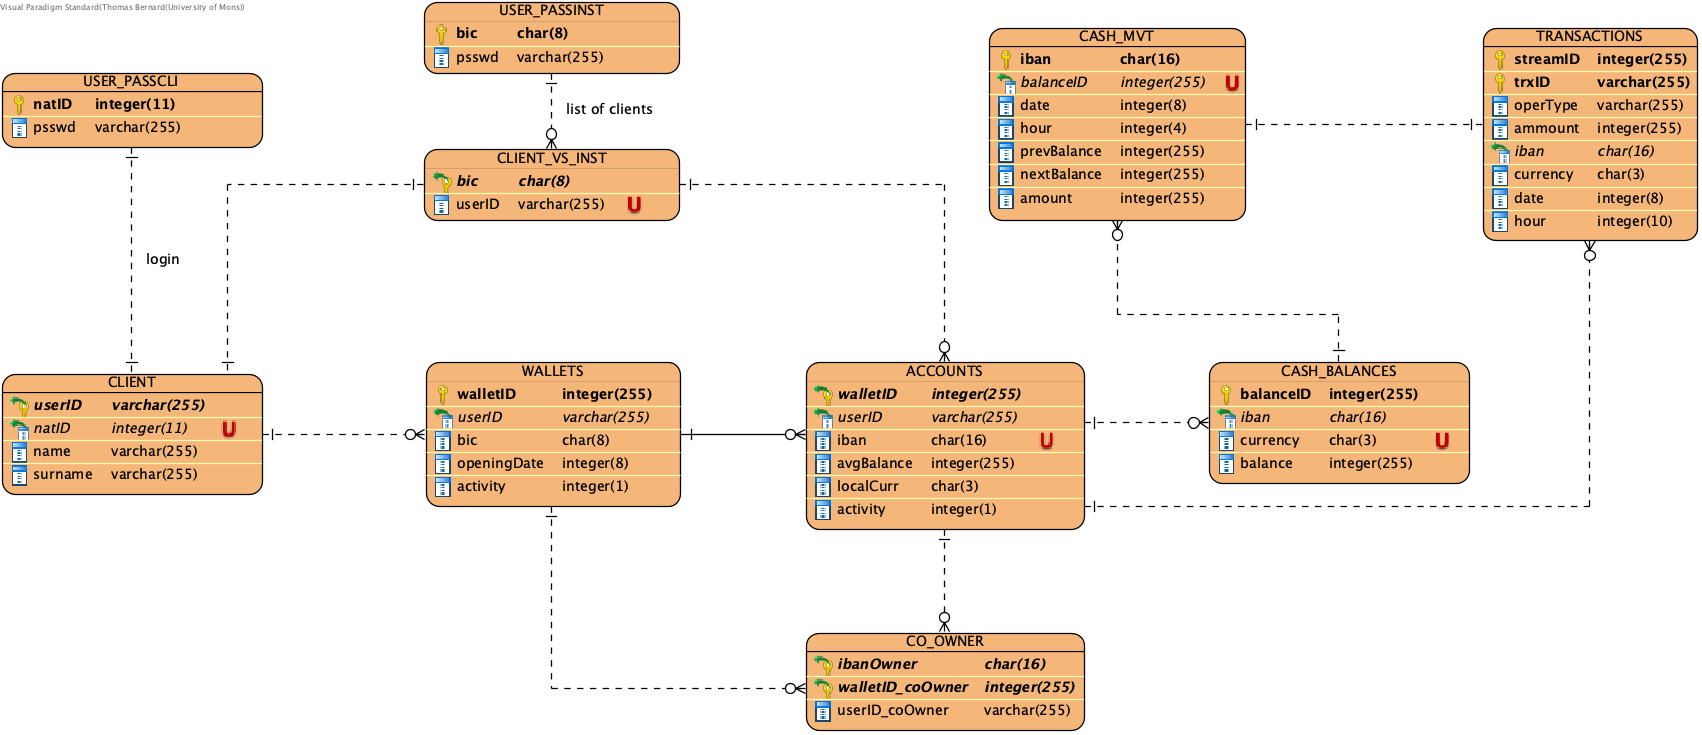
\includegraphics[scale=0.4]{ressources/photos_diagrammes/erd.png}
		\caption{Diagramme d'entité-relation de l'application.}
	\end{figure}
	
	\paragraph{Tables utilisateurs :}
	Pour notre base de données nous avons essayé de séparer au mieux les tables afin que celles-ci restent simples de compréhension et faciles d'accès. Nous avons une table \textbf{USER\_PASSCLI} qui sert de table d'authentification. Elle contient le mot de passe \textbf{psswd} ainsi que le numéro de registre national de l'utilisateur \textbf{natID} si les deux correspondent alors on peut accéder à la table \textbf{CLIENT} qui contient quant à les informations personnelles du client ainsi que son nom d'utilisateur \textbf{userID}.
	
	\paragraph{Tables des institutions :} Afin que les insitutions n'aient pas accès à la notion de portfeuilles nous avons introduit 2 tables qui leurs sont propres et qui permettent de faire le lien entre les clients de la table \textbf{CLIENT} et leurs produits financiers de la table \textbf{ACCOUNTS}.
	
	\medskip
	
	La table \textbf{USER\_PASSINST} est à l'image de la table \textbf{USER\_PASSCLI} une table d'authentification pour les institutions à l'aide de leur identifiant \textbf{bic}. 
	
	\medskip
	
	La table \textbf{CLIENT\_VS\_INST} associe chaque client et institution si pour un \textbf{userID} il possède au moins un produit financier dans l'insitution. Lorsqu'un \textit{wallet} est créé le \textbf{userID} du client ainsi que le \textbf{bic} de l'institution dans lequel il est créé sont ajoutés à la table ce qui permet ainsi à l'instution de récupérer la liste de ses clients assez aisément à l'aide de cette table. De plus elle peut ensuite se servir du \textbf{userID} afin de récupérer la liste des produits du client (table \textbf{ACCOUNTS} ainsi que ses informations personnelles (table \textbf{CLIENT}).
	

\end{document}
